\section{运动控制与仿真}
机器人关节控制是指对机器人的各个关节进行精确定位和运动控制,使机器人能够完成各种任务的过程。在先前的部分,我们小组已经对ABB-IRB-1200型号的机器人进行了一个较为逼真的建模和设计,这一部分我们将讨论在虚拟环境中对其进行运动仿真和控制,以期获得我们课程所学内容的一些复现(无论是课程ME3403《机器人学》,还是ME2232《系统模型、分析与控制(A类)》,甚至是一些不是我们学院开设的课程,比如《运动控制系统》等),同时我们也希望能通过这个大作业加深我们对机器人控制科学的认识,补足在课程内由于课时原因造成的一些“不知所学”的现象。

我们想分为3个部分对这个问题进行探讨:
\begin{enumerate}
    \item \textbf{运动学的规划仿真}:这一部分主要是对我们机器人的MDH建系、旋转矩阵的变换、关节操作空间等概念有一个认知,在脱离MATLAB工具包的情况下自行对我们建立的模型进行运动控制和仿真。
    \item \textbf{动力学的控制和仿真I}:这一部分主要研究当输入为一个力矩而不是一个运动时,机器人的相关响应。以及如果我们提供一个信号,如何让机器人进行一个更加优秀的跟踪响应。
    \item \textbf{动力学的控制和仿真II}:这一部分以理论为主,我们将电机抽象成一个一阶系统模型,通过控制框图对机器人单关节的优化控制方法进行了一些调研和复现,这部分以展示为主。
\end{enumerate}

\begin{figure}[htbp]
    \centering
    
\includegraphics[width=0.8\textwidth]{Image/logo.png}
    \caption{本大作业使用的仿真软件支持}
    \label{fig:18}
\end{figure}

我们主要使用了Solidworks和MATLAB联合仿真,如图\ref{fig:18}。在“军火展示”之前,我们写了一个配置文件\textcolor{cherry}{Configuration.pdf}(附在作业提交的压缩包中),这份文件作为我们大作业的辅助项目,介绍了如何通过Solidworks + MATLAB/Simulink和Simscape/Multibody进行联合仿真。这份指导文件中还说明了我们的一些信号(比如梯形速度曲线Trapezoidal-Curve和S型速度曲线S-Curve)在Simulink中如何生成。

导入XML文件后,可以看到图\ref{fig:19}所示的页面。通过Simulink中加入一些信号模块等作为输入,可以指导我们对运动进行仿真。

\begin{figure}[htbp]
    \centering
    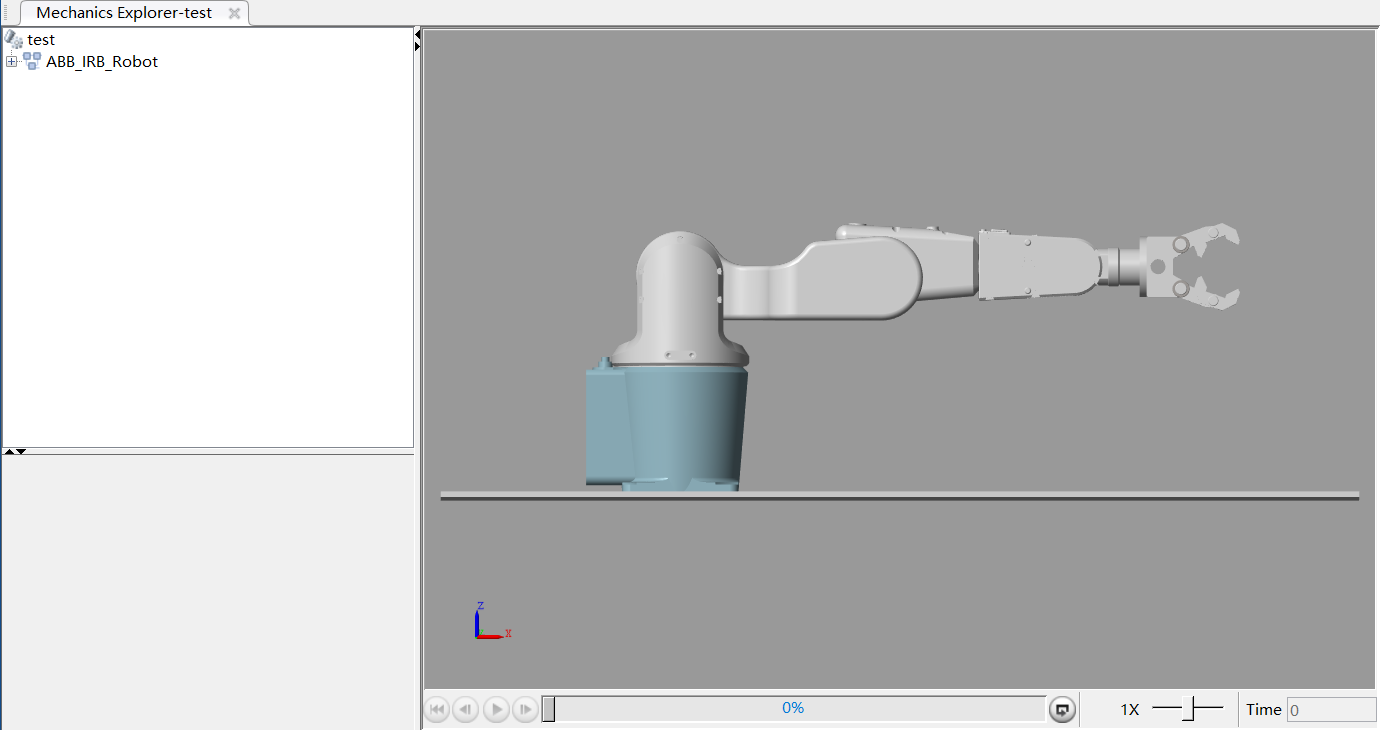
\includegraphics[width=0.8\textwidth]{Image/initial.png}
    \caption{我们小组建模的ABB-IRB-1200机器人在Simulink中的仿真页面}
    \label{fig:19}
\end{figure}

在Simulink中,一个六自由度机器人的模块化框图如下图37所示,其主要的模块有3个:Solid(刚体)、Rigid Transform (刚体坐标变换)、Revolute Joint(旋转关节)。具体的配置在文件中有说明。我们还在旋转关节中设置了传感器,反馈关节的速度、位置等信息,对应现实生活中的速度传感器和位移传感器(绝对值编码器)。

\begin{figure}[htbp]
    \centering
    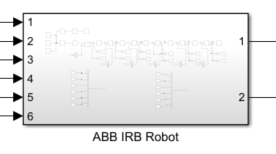
\includegraphics[width=0.4\textwidth]{Image/ABBsubsys.png}
    \caption{将机器人模型整合为6输入2输出的子系统}
    \label{fig:21}
\end{figure}

具体的模型结构如图\ref{fig:20}所示。

\begin{figure}[htbp]
    \centering
    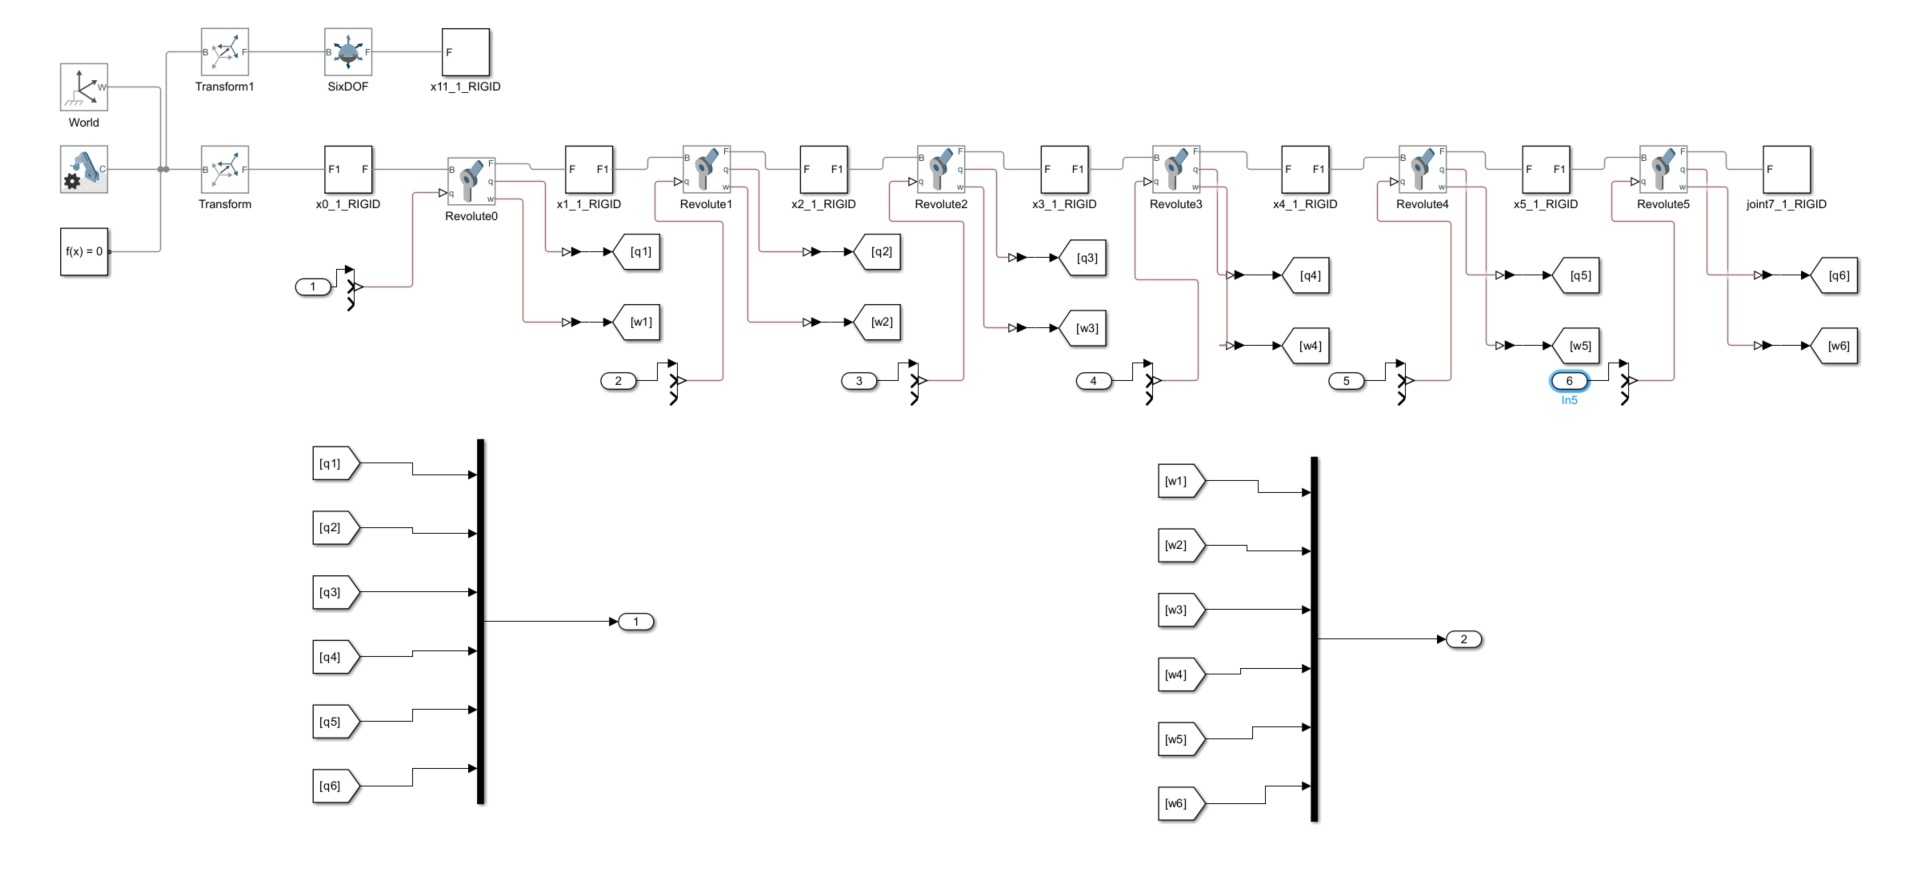
\includegraphics[width=0.7\textwidth]{Image/ABBIRB.png}
    \caption{ABB-IRB-1200机器人在Simulink中的模型结构}
    \label{fig:20}
\end{figure}

将其输入、输出通过“Mux”整合,建立一个子系统,方便面向对象的仿真操作(即我们的用户并不需要知道机器人内部的配置)。这样我们可以更好地将“面向对象”的思想纳入大作业的使用,提高我们的工程学素养,如图\ref{fig:21}所示。



\subsection{基于模型的运动学仿真}
我们将Solidworks模型导入Simscape后,把Revolute Joint的输出调节为运动信号输入模式“q”。这样的结果是模型中展示关节的运动角(直接体现运动)。如下图\ref{fig:22}所示,其余的参数比如初始角、刚度、阻尼等可以通过实际情况提供的参数进行修改。在Simulink中搭建的模型如图\ref{fig:23}所示。

\begin{figure}[htbp]
    \centering
    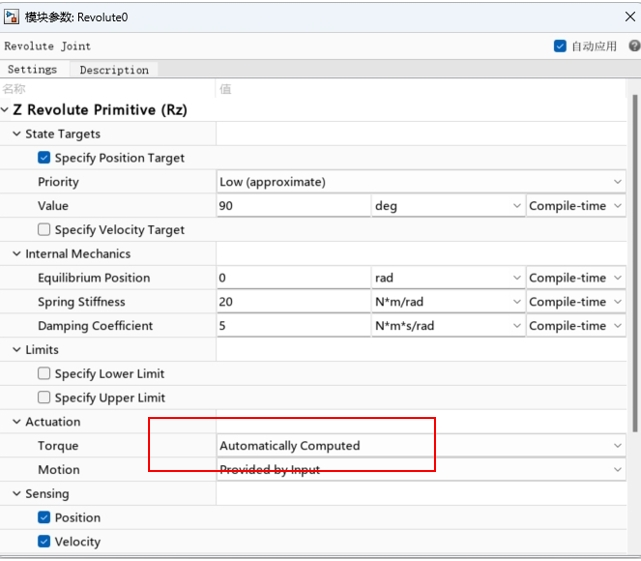
\includegraphics[width=0.4\textwidth]{Image/motion.png}
    \caption{关节运动输入模式}
    \label{fig:22}
\end{figure}

\begin{figure}[htbp]
    \centering
    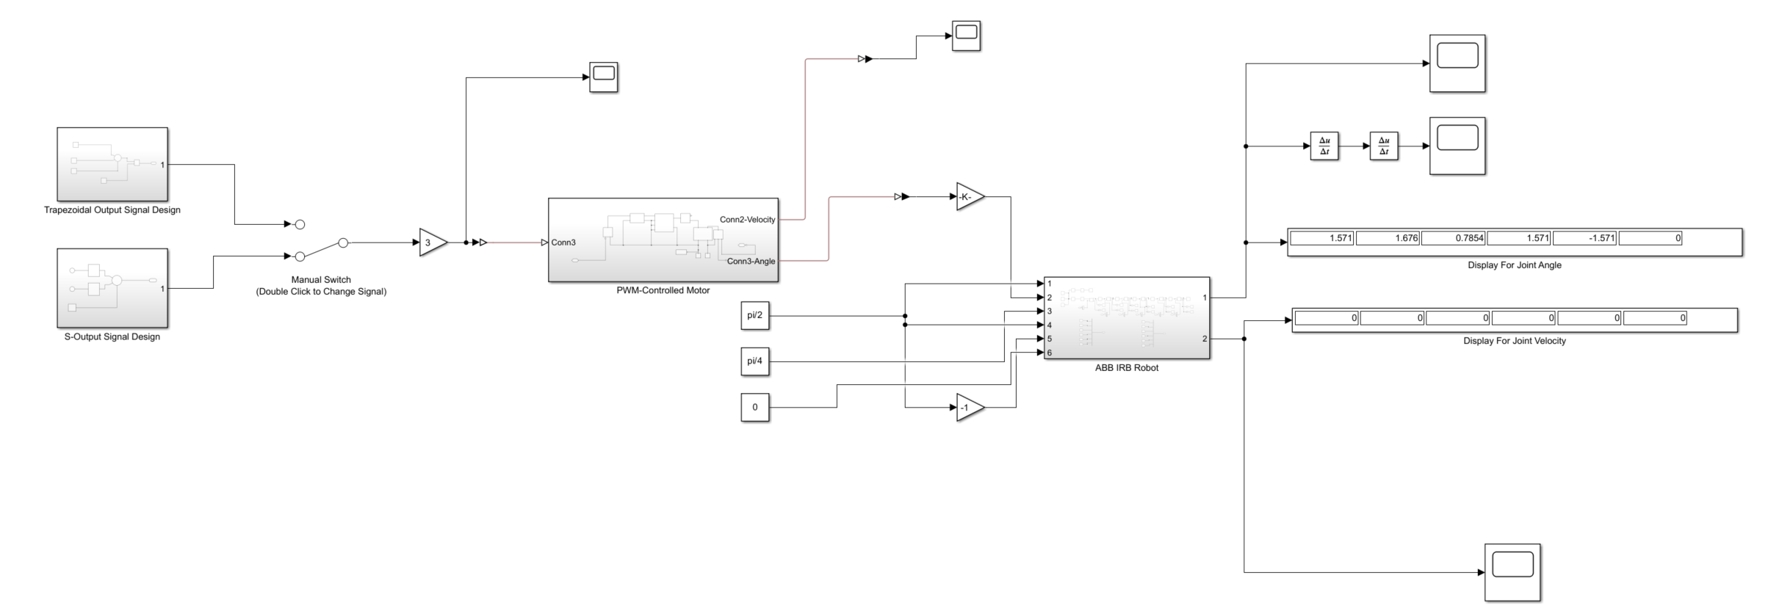
\includegraphics[width=0.8\textwidth]{Image/sim-motion.png}
    \caption{关节运动仿真模型}
    \label{fig:23}
\end{figure}

考察一个转动关节(2\#,大臂回旋),我们采用梯形运动信号输入和S型运动信号输入对机器人的运动进行模拟,可以得到关于梯形信号和S型信号的运动动画。由于报告中不方便插入视频,且转换为GIF格式后清晰度下降影响观感,因此这部分的动画可以参考附件视频或者PPT中对应的页码(Page40-Trapezoidal Signal,42-S Signal)。

\begin{figure}[htbp]
    \centering
    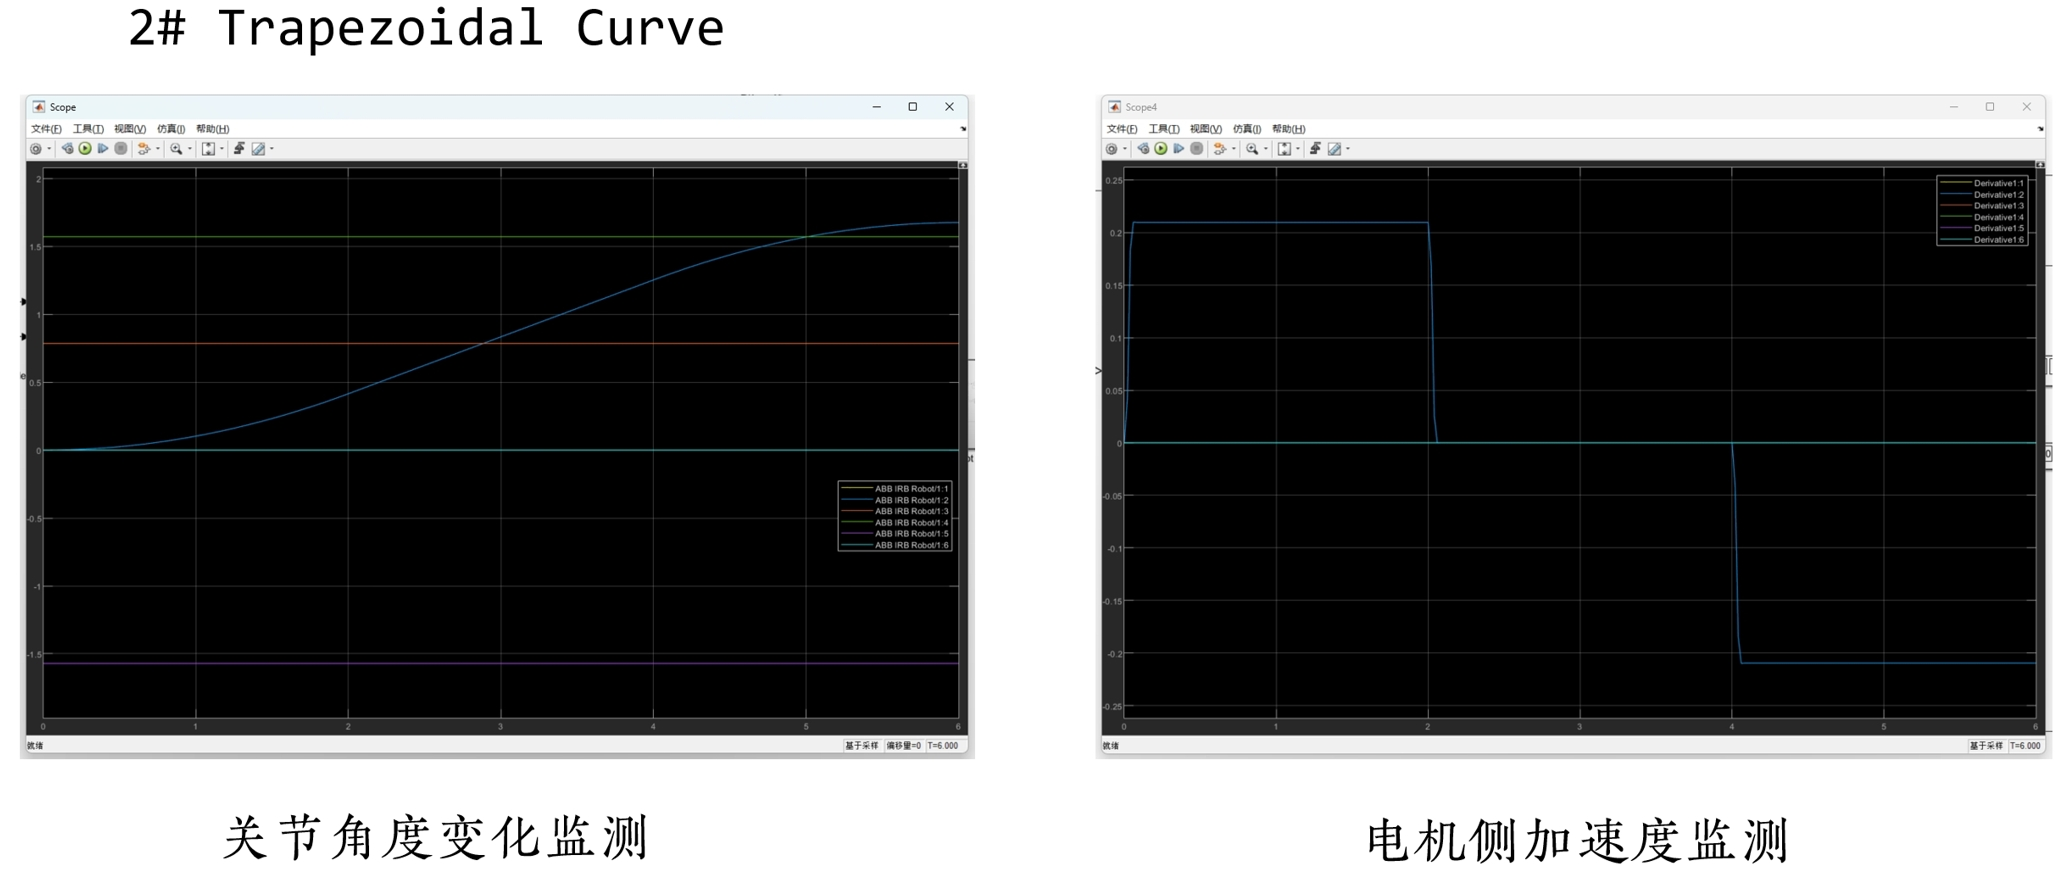
\includegraphics[width=\textwidth]{Image/fig30.png}
    \caption{梯形速度曲线下关节角度和电机侧加速度}
    \label{fig:24}
\end{figure}

对于这两种信号的应用在工程界也是有所讲究的。在工程界的电机控制中,梯形速度曲线和S型速度曲线的应用主要是为了优化电机的性能和保护机械系统。梯形速度曲线因其简单性和易于实现,广泛用于需要较快响应和精确定位的场合。这种速度曲线由加速、匀速和减速三个阶段组成,使得电机能够快速加速到目标速度,并在目标位置准确停止。然而,梯形速度曲线的加速度变化较为突兀(如图\ref{fig:24}所示),在实际的工程过程中由于工件的刚性可能会引起机械系统的振动和冲击,从而导致磨损和噪音。


相比之下,S型速度曲线则通过逐渐变化的加速度来平滑速度变化,如图\ref{fig:25}所示。显著减少了机械系统的冲击和振动。S型速度曲线的平滑过渡使其非常适合于需要高平稳性的应用,如精密加工和高精度运动控制场合,尽管其实现相对复杂且计算量较大。因此在梯形速度曲线和S型速度曲线的选择中,应用和需求通常要权衡。实际机器人的响应速度、定位精度以及系统的机械负载和寿命都是重要的考察因素。

\begin{figure}[htbp]
    \centering
    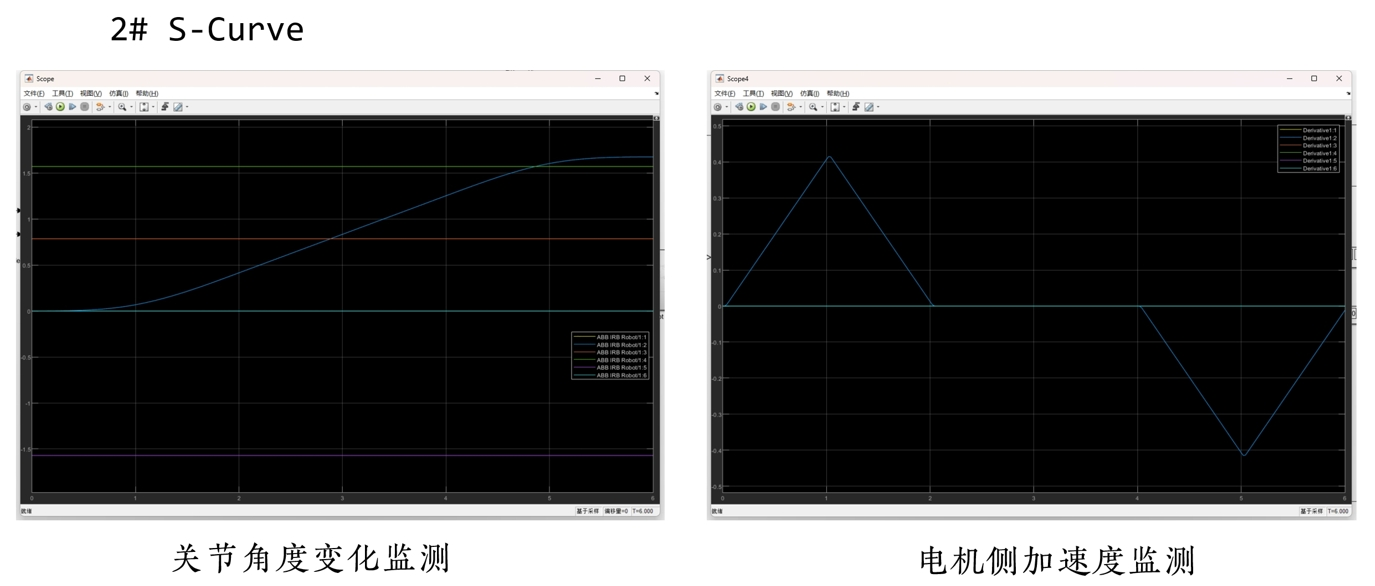
\includegraphics[width=\textwidth]{Image/fig31.png}
    \caption{S型速度曲线下关节角度和电机侧加速度}
    \label{fig:25}
\end{figure}

当然,我们也可以用一些诸如正弦、阶跃等常规的模块来构造信号观察运动,还可以采用自己设计的信号。在前面提到的运动学计算里,我们可以通过DrawCircle(Center, Radius, Face)函数来设计一个空间中的平面圆。通过求解并定义运动点数(比如200)我们能得到函数返回值q矩阵(200*6)。通过Simulink的“From Workspace”模块导入数据,并在左侧增广一个时间序列t(200*1),即可做出相应的运动(运动过程视频参见PPT或附件),机器人各关节角度如图\ref{fig:26}所示。

\begin{figure}[htbp]
    \centering
    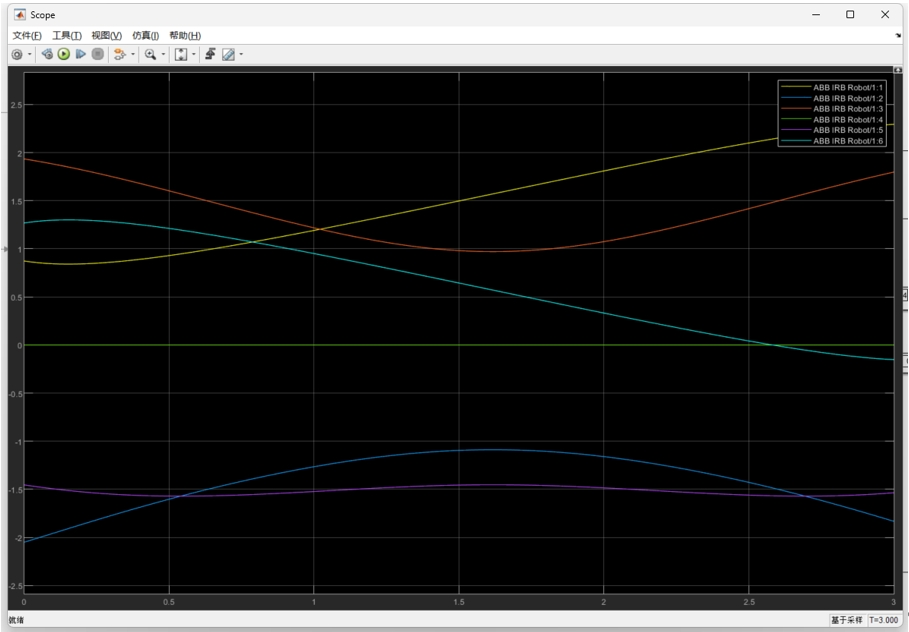
\includegraphics[width=0.5\textwidth]{Image/fig32.png}
    \caption{自定义运动下关节角度和电机侧加速度}
    \label{fig:26}
\end{figure}
\newpage
\subsection{基于模型的动力学仿真及PID控制}
在Simulink中进行机器人动力学仿真是一个复杂而庞大的过程,我们将图39所示的旋转关节参数设置中改为“Torque-Provided by Input”,如图\ref{fig:27}所示。这样相当于在旋转关节输入的是一个力矩(此处我们不考虑电机)。在前面动力学的分析中,我们通过“牛顿-欧拉”方法以及五次多项式可以规划出两点之间机器人的运动轨迹。与运动学仿真类似,在Simulink中可以输入以上计算结果的力矩进行运动仿真,当然,也可以输入一些常数(可以认为是常力矩值)来对系统进行一些测试。

\begin{figure}[htbp]
    \centering
    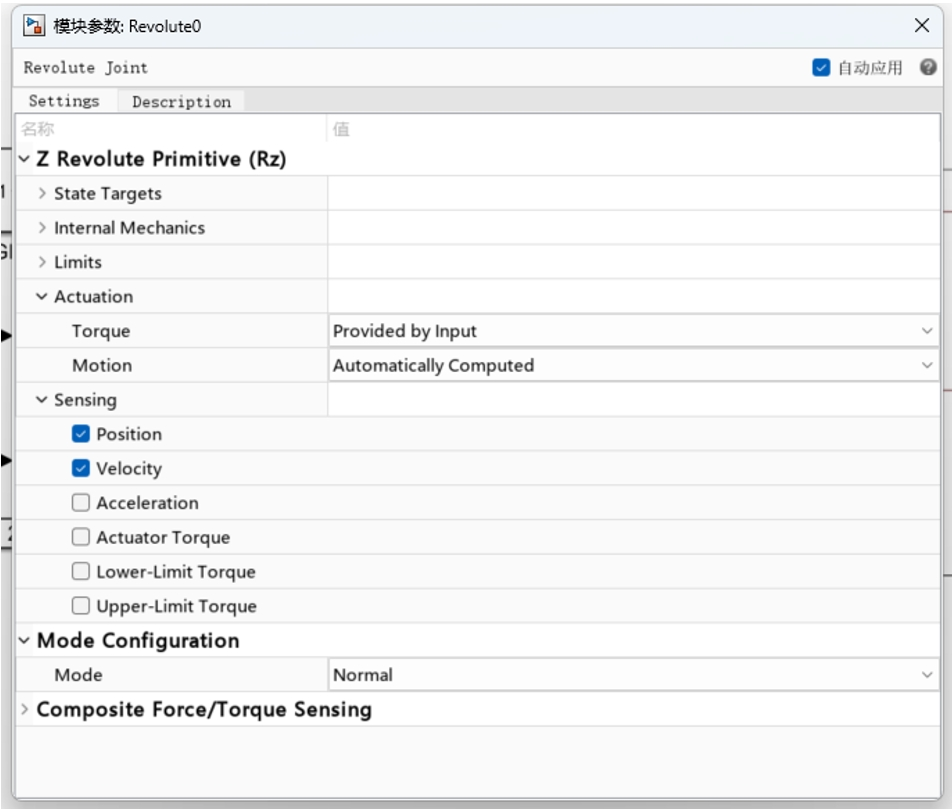
\includegraphics[width=0.4\textwidth]{Image/fig33.png}
    \caption{力矩输入模式}
    \label{fig:27}
\end{figure}

由于实际过程的动力学参数、机械结构参数、电机运动参数以及工况等因素过于多和复杂,我们的仿真不可能做到完美符合预期。因此我们从控制角度入手——通过末端绝对值编码器的反馈的位置信号,以期快速准确地达到预定的位置。对于许多机器人应用来说,控制系统的主要目标是确保关节达到预定的角度,而不需要严格的动力学模型。即使不考虑动力学,简单的PID控制器可以通过调节关节角度的误差来实现预期的定位。虽然PID控制器没有明确考虑动力学方程,但在某些情况下,适当调节PID增益可以隐式地补偿机器人系统的动力学特性。特别是在低速和低负载条件下,动力学效应对控制精度的影响较小,PID控制器能够提供足够的性能。引入PID后,系统局部如下图\ref{fig:28}所示。

\begin{figure}[htbp]
    \centering
    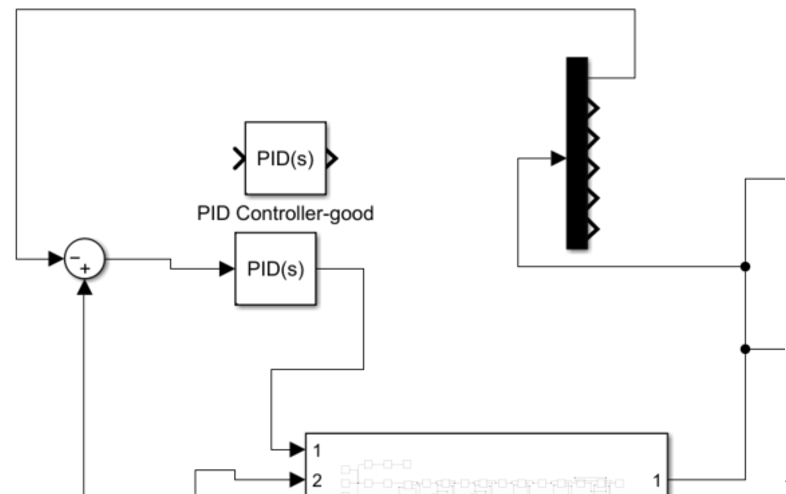
\includegraphics[width=0.6\textwidth]{Image/fig34.png}
    \caption{PID控制器的局部}
    \label{fig:28}
\end{figure}

由于实际过程的动力学参数、机械结构参数、电机运动参数以及工况等因素过于多和复杂,我们的仿真不可能做到完美符合预期。因此我们从控制角度入手——通过末端绝对值编码器的反馈的位置信号,以期快速准确地达到预定的位置。对于许多机器人应用来说,控制系统的主要目标是确保关节达到预定的角度,而不需要严格的动力学模型。即使不考虑动力学,简单的PID控制器可以通过调节关节角度的误差来实现预期的定位。虽然PID控制器没有明确考虑动力学方程,但在某些情况下,适当调节PID增益可以隐式地补偿机器人系统的动力学特性。特别是在低速和低负载条件下,动力学效应对控制精度的影响较小,PID控制器能够提供足够的性能。引入PID后,系统局部如图\ref{fig:28}所示。

\begin{figure}[htbp]
    \centering
    \subfigure[Without PID]{
    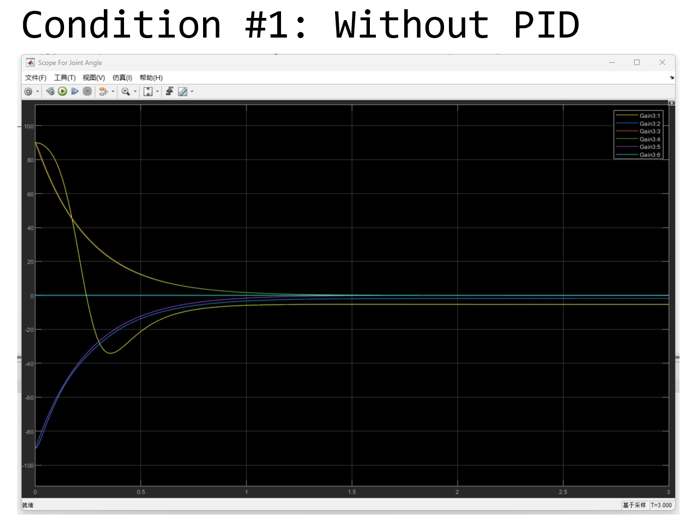
\includegraphics[width=7cm]{Image/fig35.png}
    \label{fig:29}
    }
    \quad
    \subfigure[$K_p=200,K_i=10,K_d=0$]{
    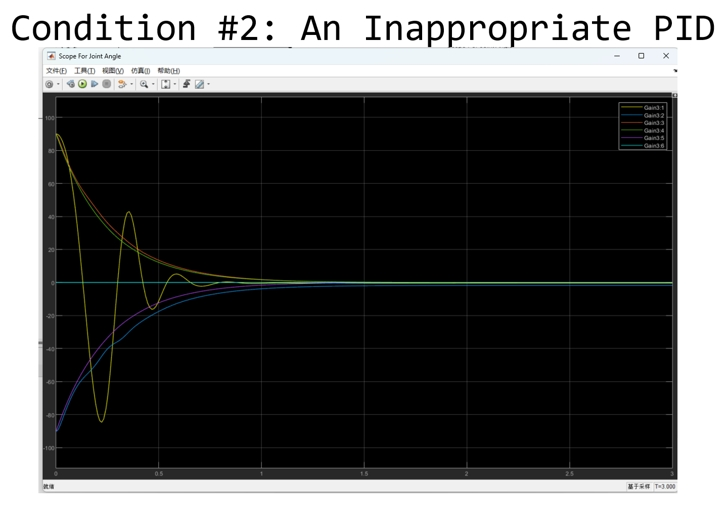
\includegraphics[width=8cm]{Image/fig36.png}
    \label{fig:30}
    }
    \quad
    \subfigure[$K_p=13.5,K_i=2,K_d=13.5$]{
    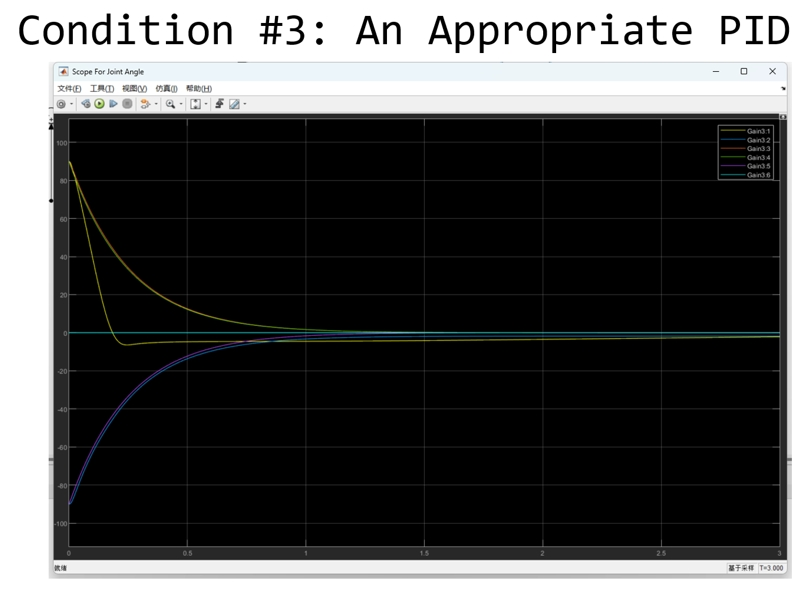
\includegraphics[width=7cm]{Image/fig37.png}
    \label{fig:31}
    }
    \caption{不同PID参数下的系统响应效果}
    \label{fig:28}
\end{figure}

没有PID控制的情况如图\ref{fig:29}所示。可以看到一号关节(黄色曲线)是一个典型的欠阻尼曲线,而且存在稳态误差。我们将此作为基本运动,对其进行调制。在图\ref{fig:30}中,我们使用了一个“不太优秀”的PID控制器,这个控制器的参数为$K_p=200,K_i=10,K_d=0$,它显著地增大了超调量,而且多了很多振荡不平衡的因素,不过最后稳态误差消除做的还比较理想。

在图48中我们调试出了一个较为优秀的PID控制器,该控制器在响应速度、稳态误差方面都做的很好,其$K_p=13.5,K_i=2,K_d=13.5$。具体的运动细节通过仿真很容易辨识出来,可以看到较差的控制器下振荡是很明显的,而表现优秀的PID使得关节响应准确、迅速。

\subsection{工业界机器人控制理论及部分复现}

这一部分我们主要从工业界主流的机器人控制理论出发,探讨工业界常见串联机械臂的动力学和控制问题。机器人的关节控制通常是“三环”,如图\ref{fig:32}所示。这三层控制环路层层递进,通过内层环路提供更快速和精确的控制响应,确保机器人关节运动的稳定性和准确性。

\begin{figure}[htbp]
    \centering
    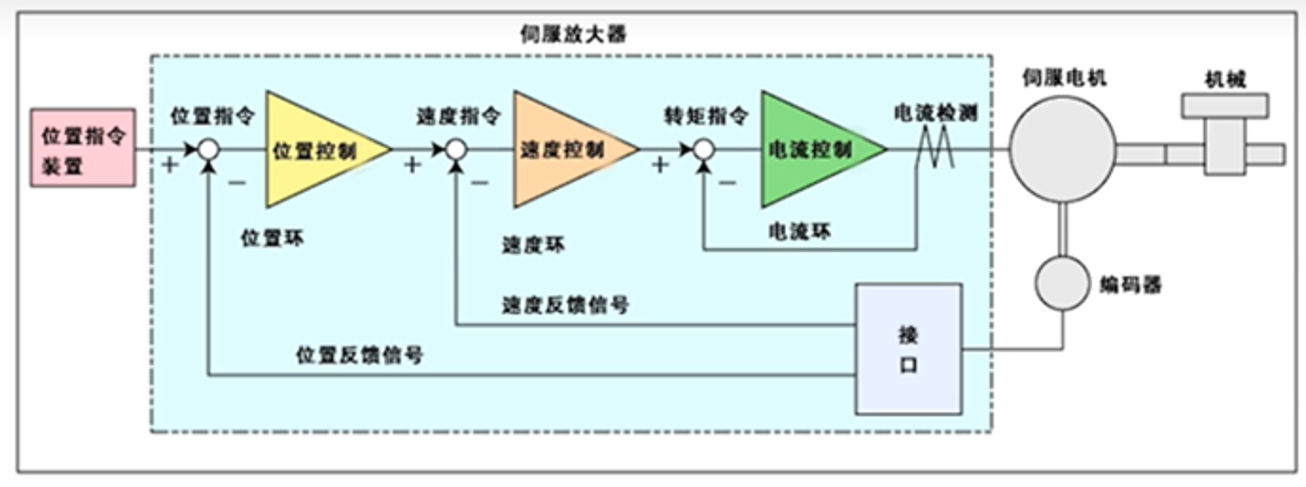
\includegraphics[width=0.8\textwidth]{Image/fig38.png}
    \caption{机器人关节控制的“三环”结构}
    \label{fig:32}
\end{figure}

\textbf{电流环控制}:电流环控制是机器人关节控制的最内层环路,主要用于控制电机的电流。通过调节电流,可以直接影响电机的转矩,从而实现精确的力矩控制。电流环通常使用电流传感器反馈实际电流值,并与期望值进行比较,调整电压输出以减少误差,确保电机产生所需的力矩。这不是《机器人学》以及控制课的重点研究内容。

\textbf{速度环控制:}速度环控制是基于电流环之上的一个控制层,用于控制电机的转速。速度环使用速度传感器(如编码器)反馈电机的实际转速,与设定的目标速度进行比较,生成一个速度误差信号。这个误差信号再经过调节器(如PI调节器)处理,输出一个电流设定值,驱动电流环以调整电机的转速,实现对速度的精准控制。

\textbf{位置环控制}:位置环控制是机器人关节控制的最外层环路,负责控制关节的位置。通过位置传感器(如编码器或光学尺)反馈实际关节位置,与目标位置进行比较,生成位置误差信号。位置误差信号经过调节器处理,输出一个速度设定值,传递给速度环。速度环再将该设定值转化为电流设定值,逐层传递下去,最终实现对关节位置的精确控制。

因而我们本次大作业主要考虑速度环和位置环的控制模型搭建和测试。对于一个机器人关节,动力学上有一个优雅而简洁的方程进行描述:

\begin{equation}
    Q=M\left( q \right) \ddot{q}+C\left( q,\dot{q} \right) \dot{q}+F\left( \dot{q} \right) +G\left( q \right) +J\left( q \right) ^Tf
\end{equation}

式(39)中,Q代表广义驱动力,M是关节空间惯量矩阵,C是科里奥利力和向心力耦合矩阵,G是重力负荷,f是摩擦力,J是雅可比矩阵。在Peter Corke的机器人学工具包中,通过SerialLink.rne()方法(牛顿欧拉递归)可以从基座开始推算每个关节应该有的扭矩,具有O(N)的计算复杂性。

考虑一个电流控制的电机:
\begin{equation}
    \left\{ \begin{array}{c}	i=K_au\\	J_m\dot{\mathrm{\omega}}+B\omega +\mathrm{\tau}_c\left( \mathrm{\omega} \right) =K_mK_au\\\end{array} \right.
\end{equation}

其中$K_a$是运算放大器的跨导,$K_m$是电机的扭矩常数,电机的动力学模型可简化。其中$J_m$是电机的总惯量, $B$是电机的粘性摩擦系数,$\tau_c$是电机的库伦摩擦力矩。如果忽略库伦摩擦阻力项,对上式进行Laplace变换,可以得到:

\begin{equation}
    \left\{
        \begin{aligned}
            &sJ\Omega(s) + B\Omega(s)=K_mK_aU(s) \\
            &\frac{\Omega\left( s \right)}{U\left( s \right)}=\frac{K_mK_a}{J_ms+B}
        \end{aligned}
    \right.
\end{equation}

因此把电机简化为一个一阶系统模型。

\subsubsection{速度环控制}
通过上述分析,我们给电机的指令为:
\begin{equation}
    u^*=K_v(\dot{q}^*-\dot{q})
\end{equation}

因此搭建了一个速度环控制系统模型vloop.slx,如图\ref{fig:33}所示。

\begin{figure}[htbp]
    \centering
    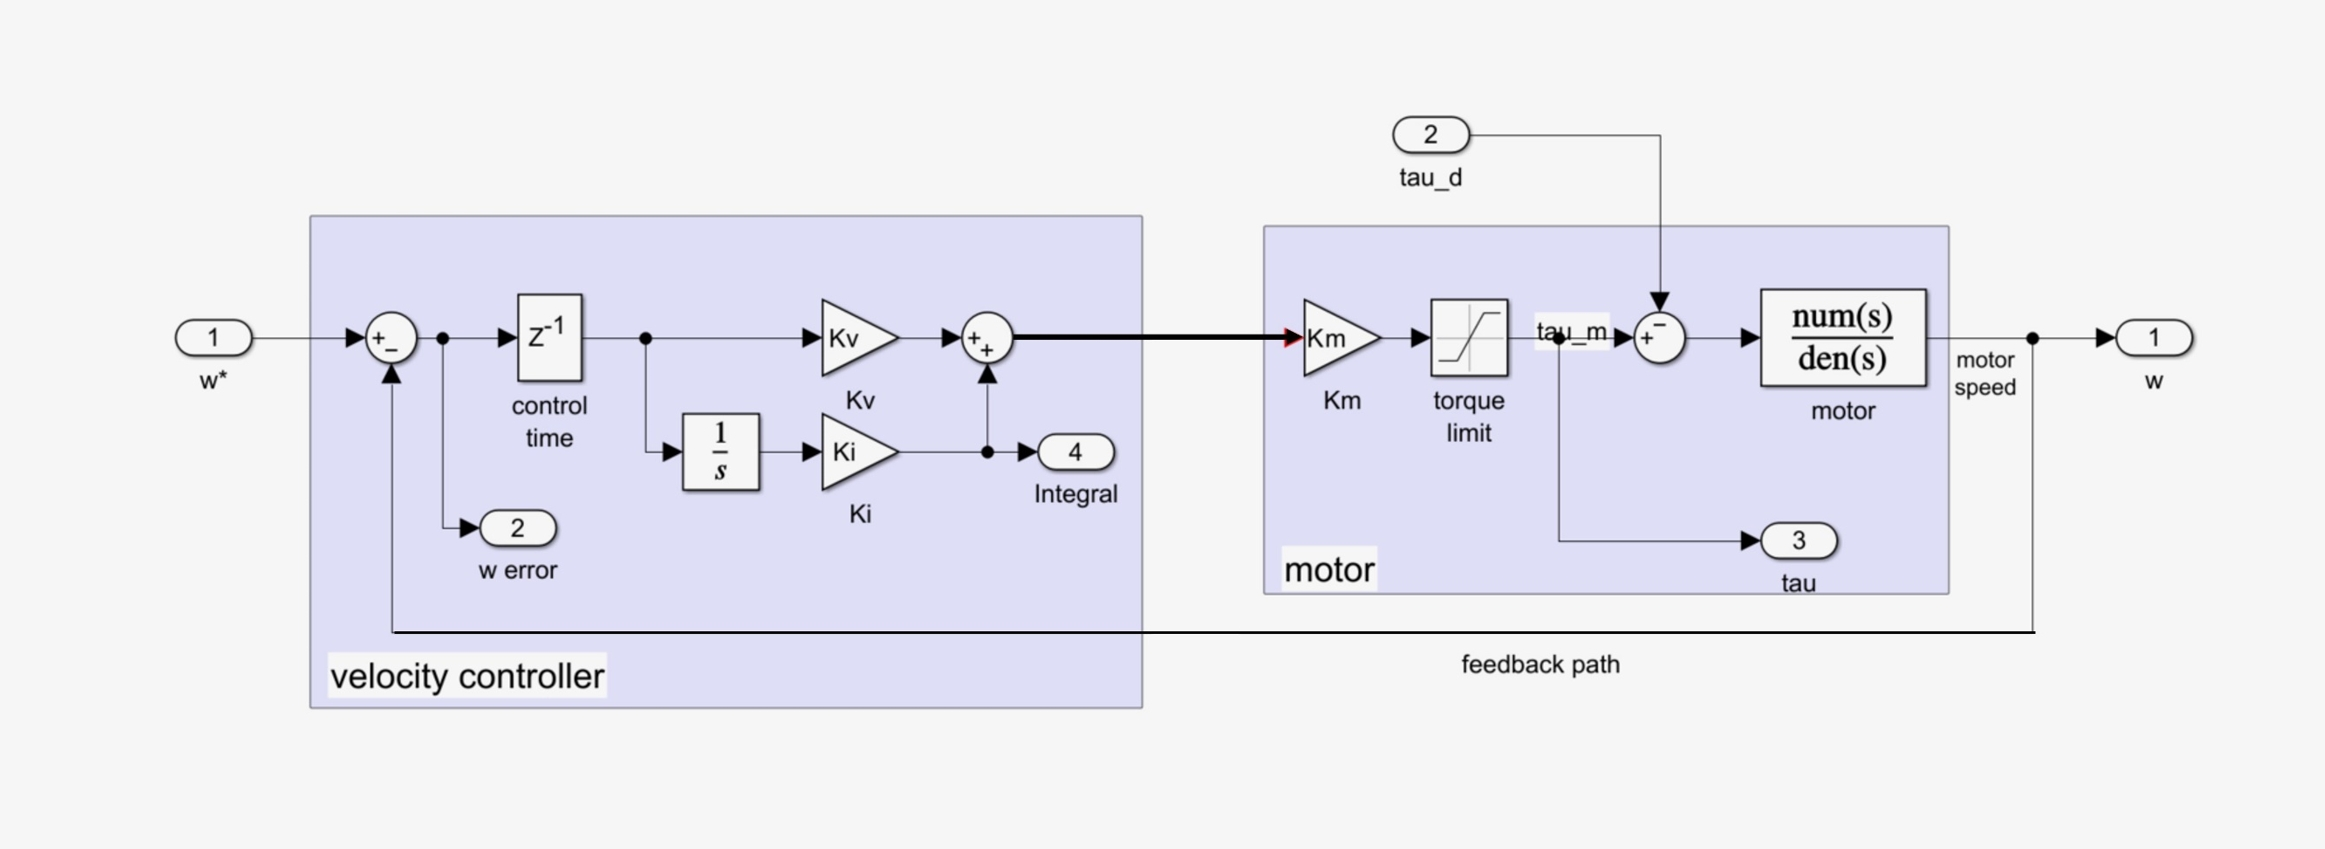
\includegraphics[width=0.8\textwidth]{Image/vloop.png}
    \caption{速度环控制系统模型}
    \label{fig:33}
\end{figure}

将速度环封装在测试模型中(如图51所示),外部保留速度期望(desired speed)、干扰力矩($\tau_d$)的输入口,同时添加几个示波器用于检测关节速度和跟踪误差。需要一提的是,在图\ref{fig:33}中我们可以看到是有 $K_v,K_i$两个参数对反馈的信号进行调节,即我们提到的PI-Controller。测试模型如图\ref{fig:34}所示。

\begin{figure}[htbp]
    \centering
    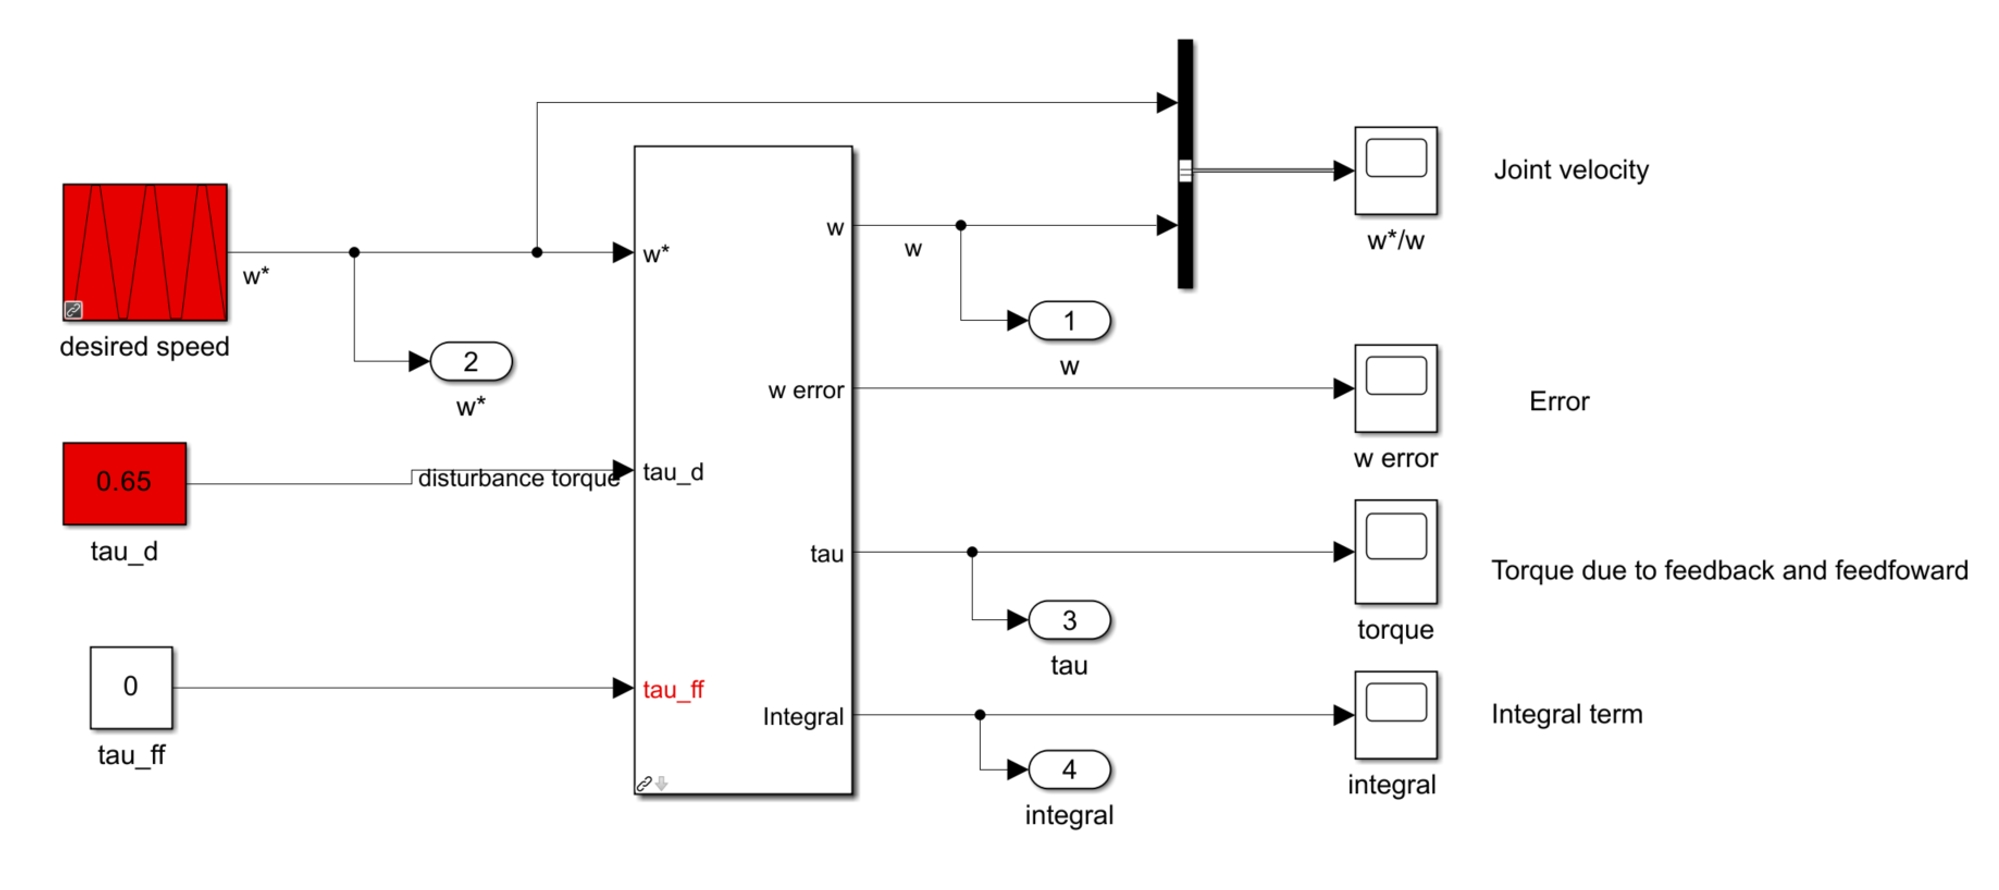
\includegraphics[width=0.8\textwidth]{Image/vloop_test.png}
    \caption{速度环控制系统测试模型}
    \label{fig:34}
\end{figure}

接着在这个模型上进行测试,第一种情况我们假设没有干扰力矩,采用之前提到的连续梯形速度信号作为输入,可以得到下图\ref{fig:35}所示的结果。其中PI控制器的参数$K_p=1,K_i=10$。可以看到速度信号的跟踪水平一般,在速度的一阶导突变的地方跟踪性能会有一定的误差,考察Error图可以发现误差较大时,可以达到$1rad/s$。

\begin{figure}[htbp]
    \centering
    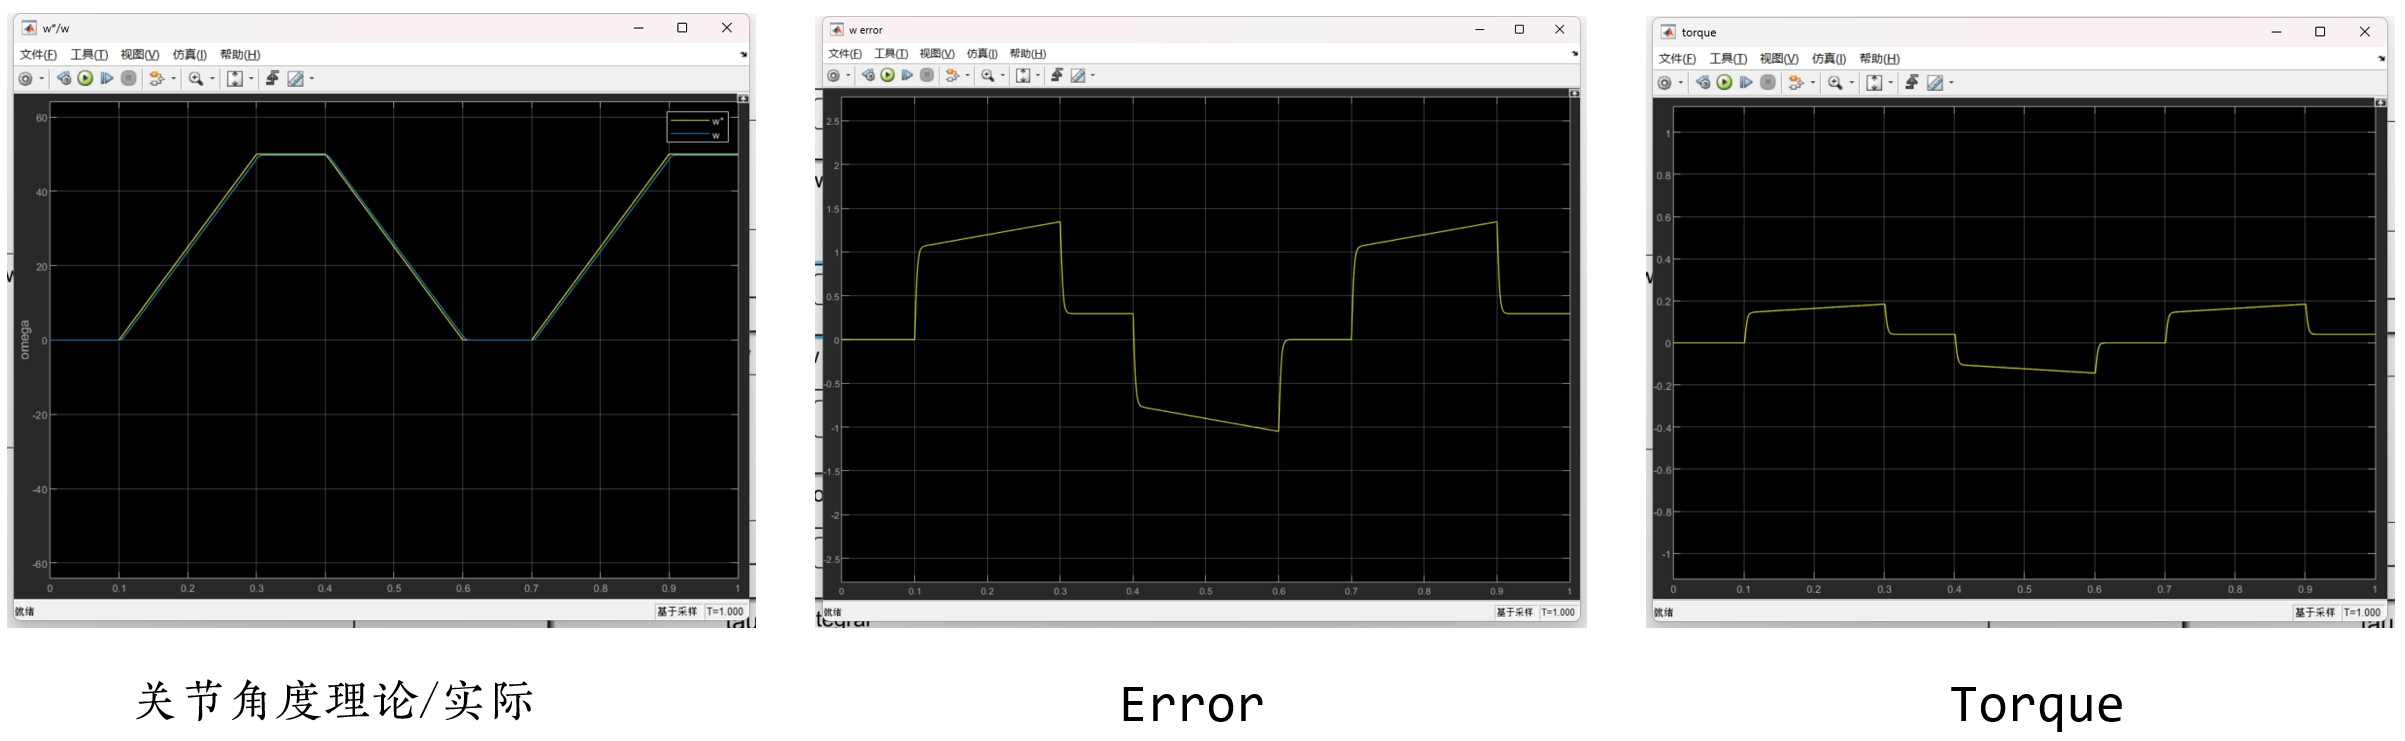
\includegraphics[width=\textwidth]{Image/fig40.png}
    \caption{零干扰力矩的速度环跟踪性能测试}
    \label{fig:35}
\end{figure}

但是对于实际的工程应用情景,机械手臂一定是存在重力作用的,因次每当我们在进行机械手臂的动力学仿真时一定要考虑重力力矩的影响。于是我们进行了第二组测试——添加干扰力矩,测试水平如图\ref{fig:36}所示。当添加的干扰力矩为$0.65N\cdot m$时跟踪误差将会更加显著($>3rad/s$),只是由于纵坐标的尺度不同,因此相对于图\ref{fig:35}其视觉上的误差更加小,实际上是更大的。

\begin{figure}[htbp]
    \centering
    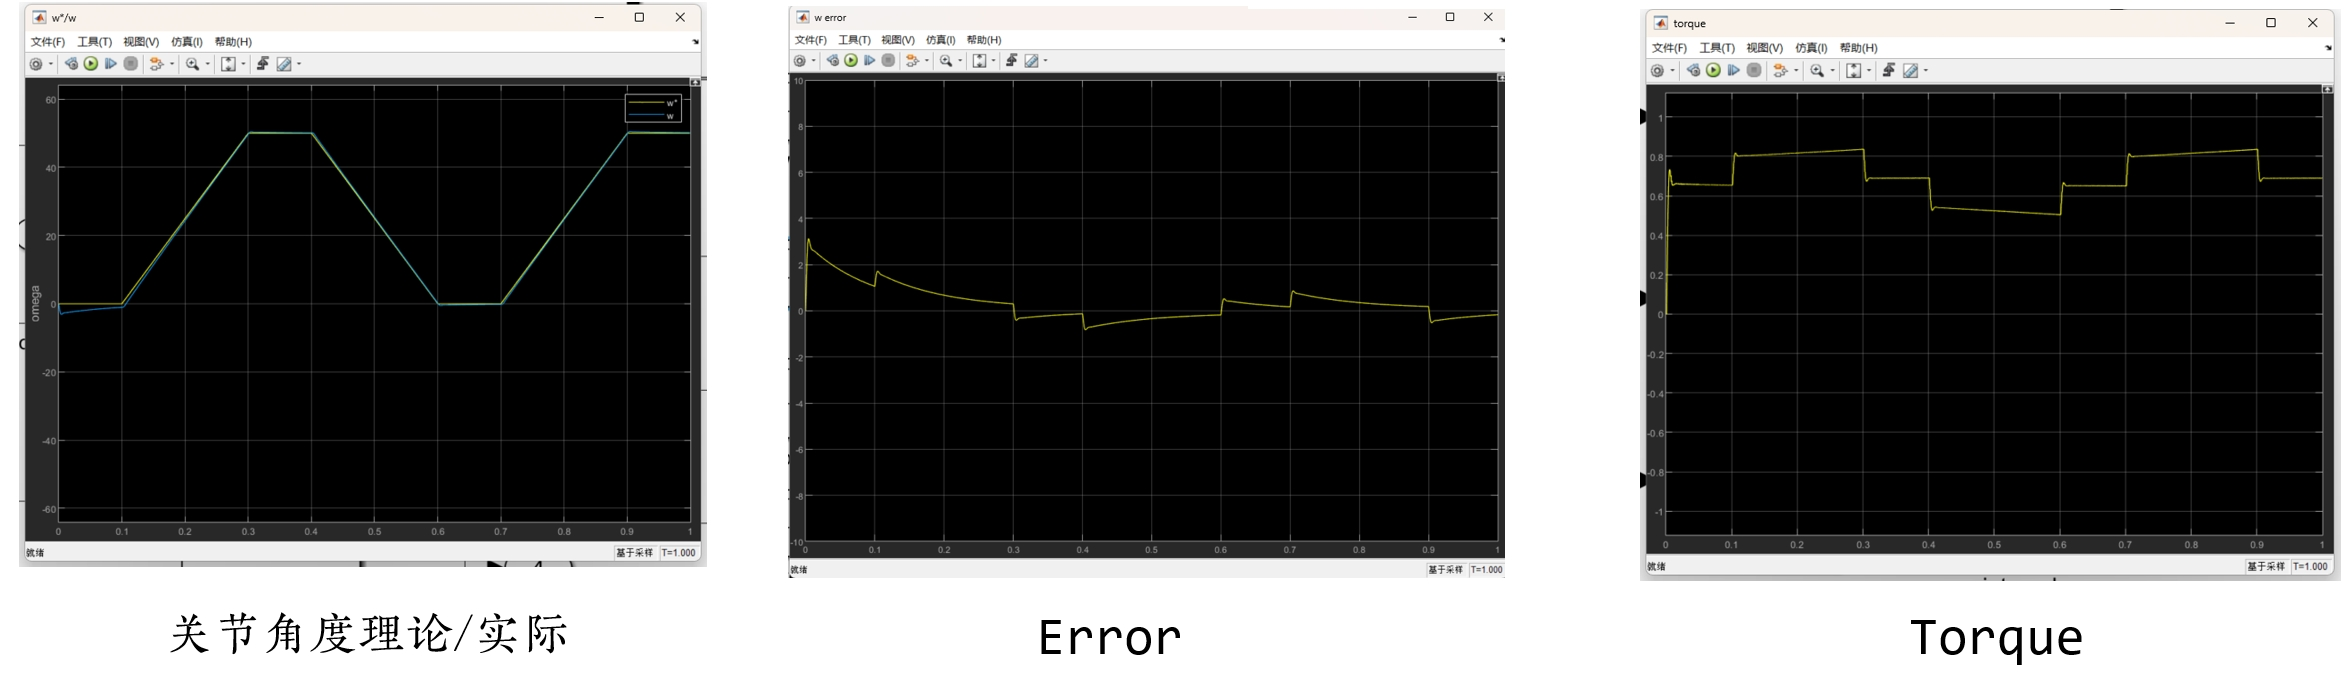
\includegraphics[width=\textwidth]{Image/fig41.png}
    \caption{有干扰力矩的速度环跟踪性能测试}
    \label{fig:36}
\end{figure}

上述过程即为我们小组对速度环控制的研究。通常在工业界内有3中方法对机器人关节运动的跟踪性能进行改善:

\begin{itemize}
    \item \textbf{增加控制器增益}:通过增加控制器的比例增益$K_p$,可以提高系统的响应速度和稳定性,减小跟踪误差。但是增益过大会导致系统不稳定,产生振荡和过冲现象,使得系统不稳定。
    \item \textbf{增加积分增益}:在模型中引入积分增益$K_i$进行改善,做成如上图\ref{fig:33}中的PI控制器Velocity Controller。此时输入信号变为
    \begin{equation}
        \begin{aligned}
           \text{Time Domain:}\quad &u^*=K_v(\dot{q}^*-\dot{q})+K_i\int_{0}^{t}(\dot{q}^*-\dot{q})dt\\
           \text{Laplace Domain:}\quad  &U^*(s)=(K_v+\frac{K_i}{s})(\dot{q}^*(s)-\dot{q}(s))\\
           & (where \quad K_i>0)
        \end{aligned}
    \end{equation}

    这样的优势是将原来的0型系统变成了一个1型系统,因此对恒定的输入表现为0误差,但相应的缺点就是由于积分环节的作用可能会产生比较大的超调量。
    \item \textbf{加入前馈法}:对于一个实际的机器人模型,不管是PUMA560还是我们建的ABB-IRB-1200,其重力的干扰并不是未知的。我们可以计算估计或者使用一些上限/下限,预测干扰并消除它。值得一提的是,即使我们设置的前馈量不准确,前馈控制也能减少干扰的浮动。\textcolor{cherry}{也许这就是前馈控制系统的魅力所在吧。}
\end{itemize}

在工业界,前两种方法我们称为“\textbf{干扰抑制}”,后一种方法称为“\textbf{力矩前馈控制}”。让我们来观察一下力矩前馈控制的效果,系统框图如图\ref{fig:37}所示。

\begin{figure}[htbp]
    \centering
    \subfigure[力矩前馈控制框图]{
    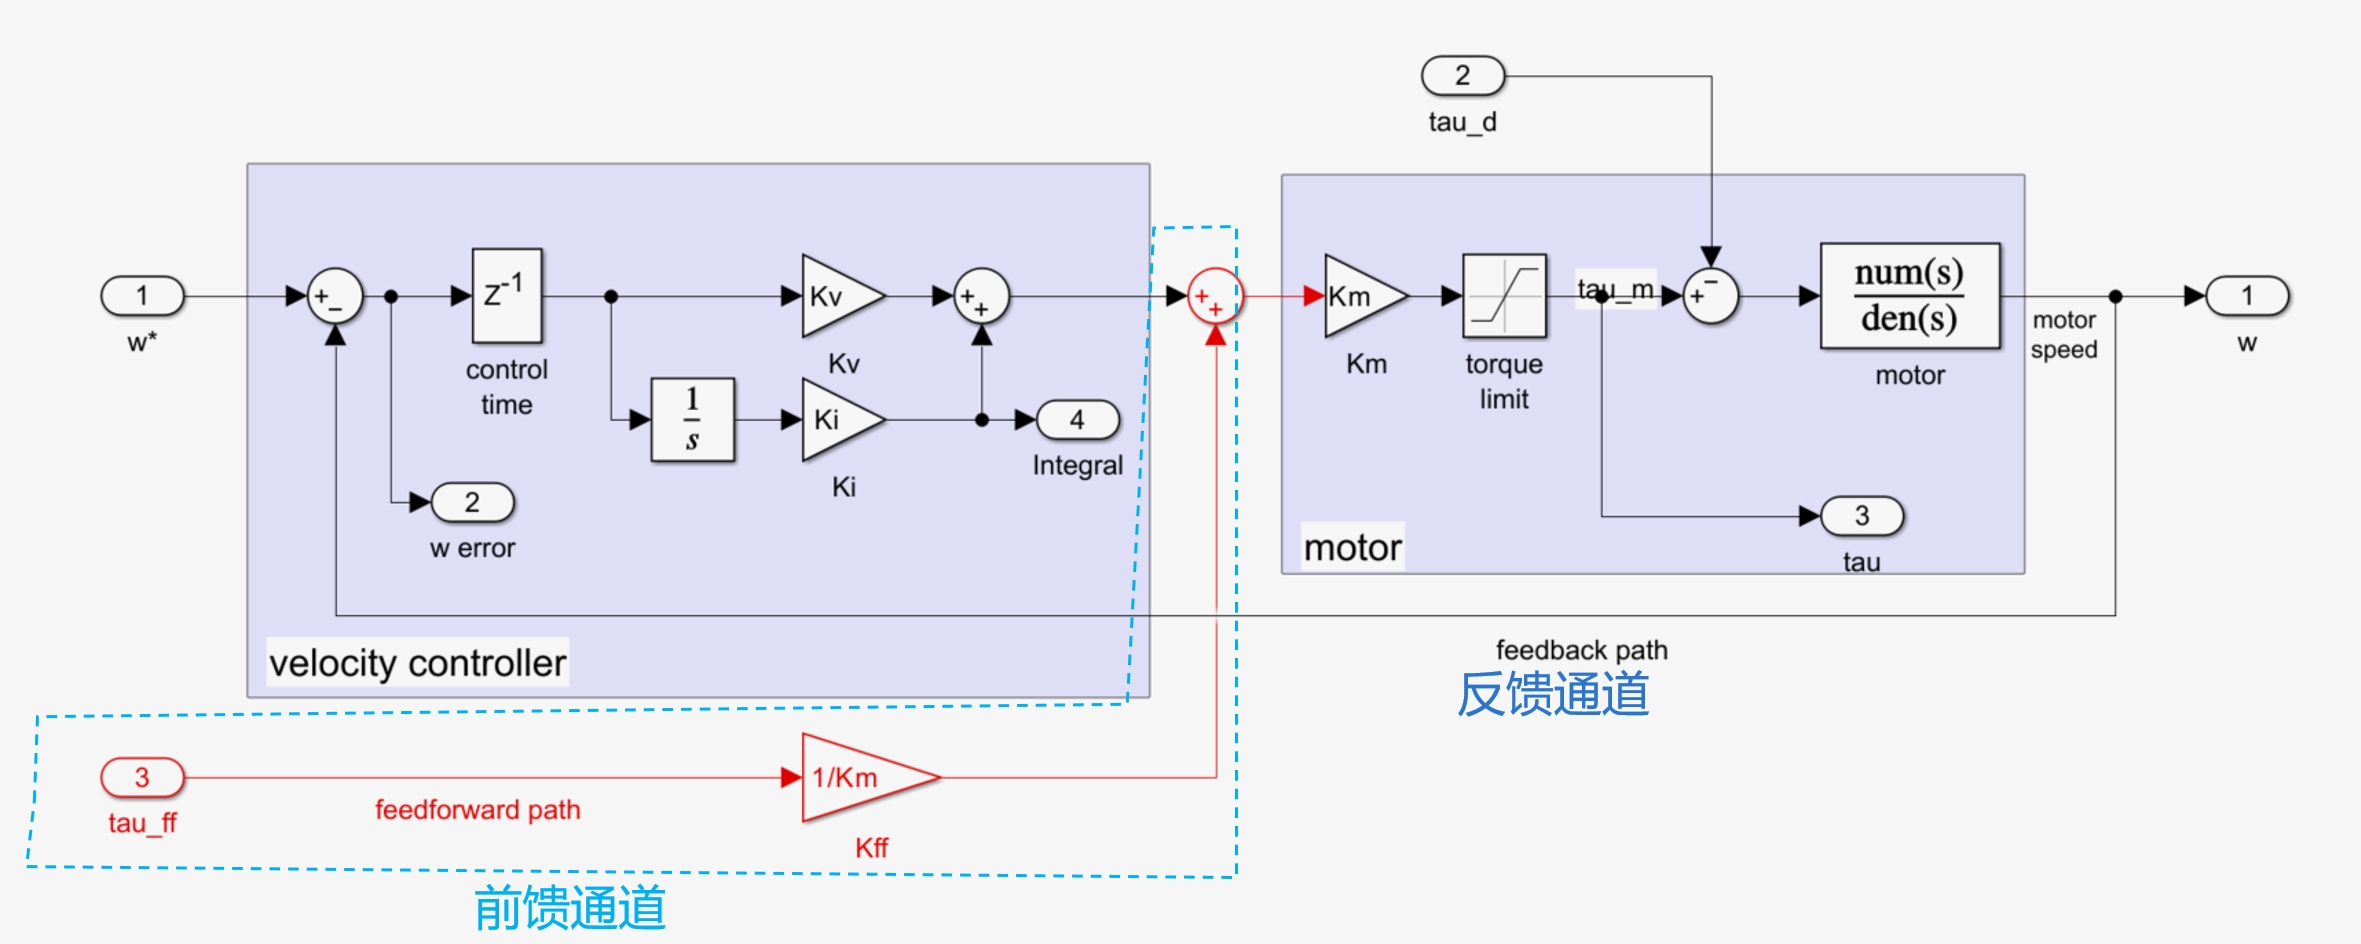
\includegraphics[width=0.45\textwidth]{Image/力矩前馈.png}
    }
    \subfigure[力矩前馈测试系统]{
    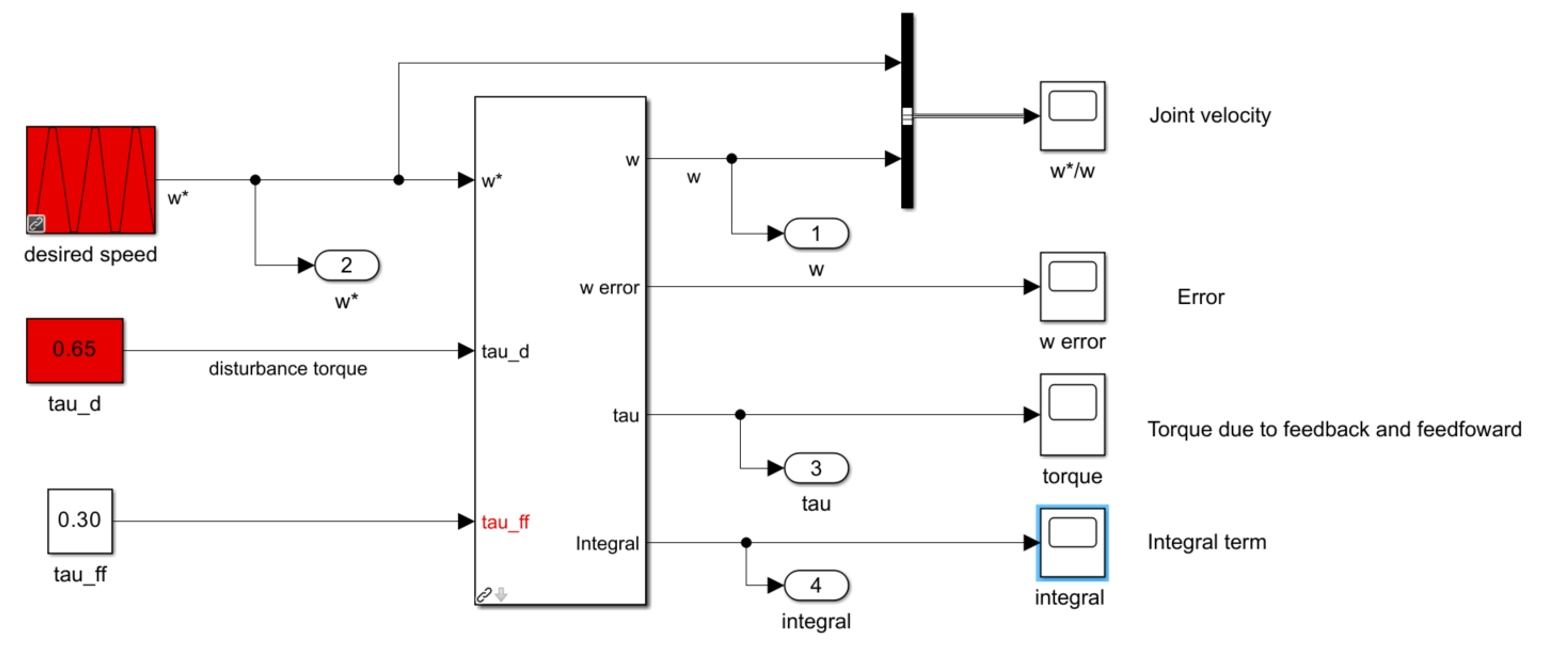
\includegraphics[width=0.45\textwidth]{Image/力矩前馈测试.png}
    }
    \caption{力矩前馈控制系统}
    \label{fig:37}
\end{figure}

在测试环节加入了0.30的前馈量$\tau_{ff}$,对于同样的控制器参数,跟踪性能展示如图\ref{fig:38}所示,对比图\ref{fig:36},可以看到Error明显减少了(此时的纵坐标尺度相同),也成功地体现了前馈控制的作用.

\begin{figure}[htbp]
    \centering
    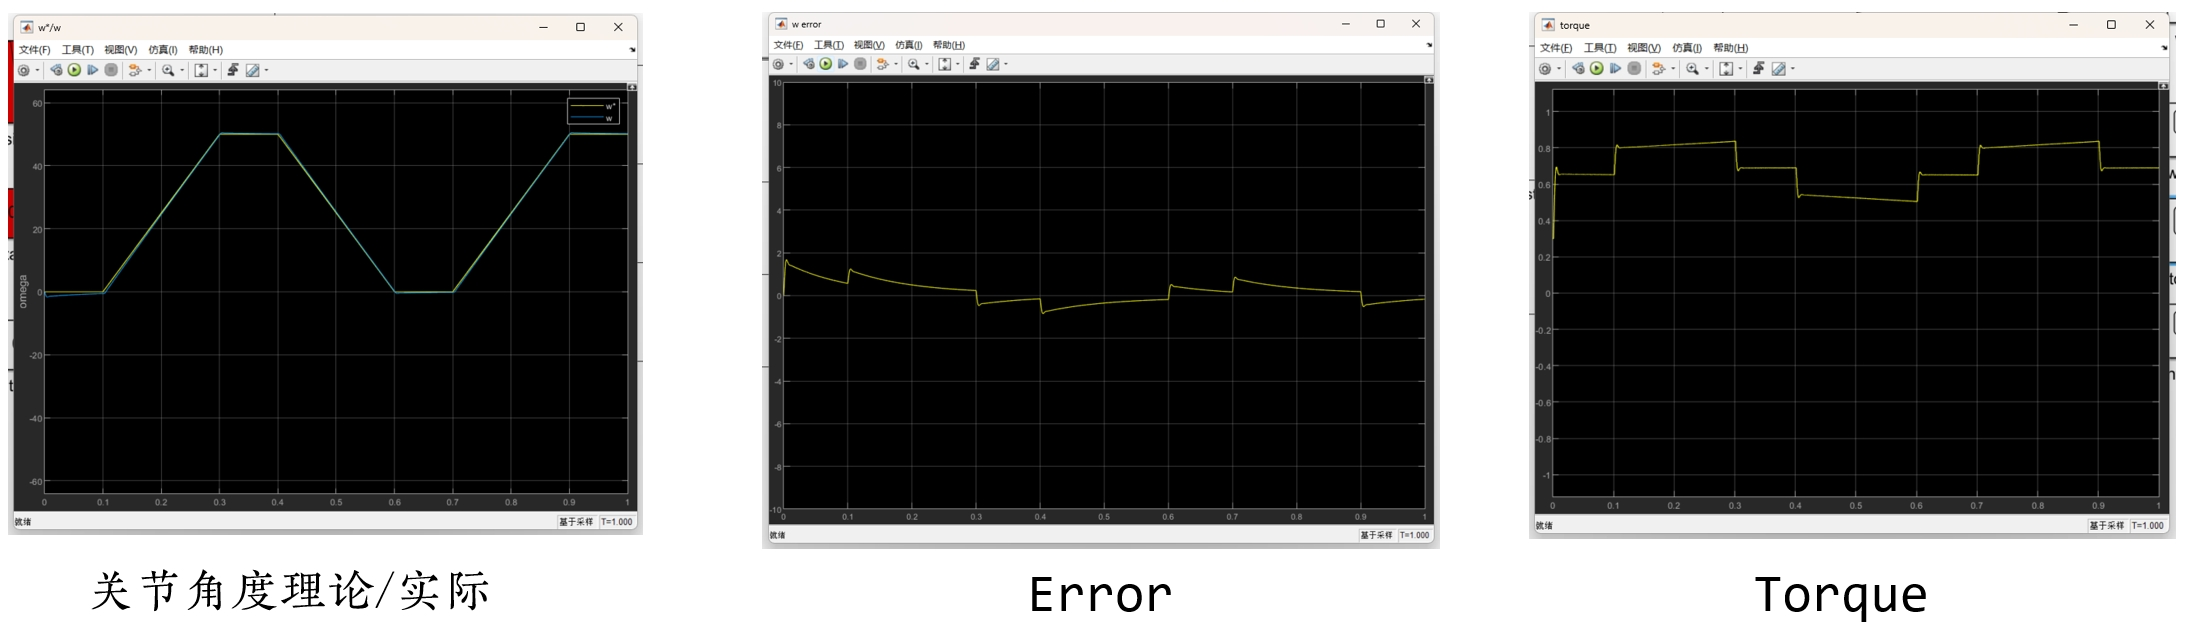
\includegraphics[width=\textwidth]{Image/fig42.png}
    \caption{力矩前馈控制速度环系统跟踪性能测试}
    \label{fig:38}
\end{figure}

\subsubsection{位置环控制}
可以这样理解:外环通过绝对值编码器检测关节位置,位置的误差为内环提供了速度要求。因此一个Ploop控制器应该嵌套了前一节中的速度环vloop,如图\ref{fig:39}所示。左上角为Ploop的外部测试,子系统ploop的结构如右下部分所示,其中包含了一个之前提到的vloop子系统。LSPB是一个集成好的轨迹发生器,规划关节1s内从0运动到1rad,并反馈回 $q,\dot{q},\ddot{q}$信息。

\begin{figure}[htbp]
    \centering
    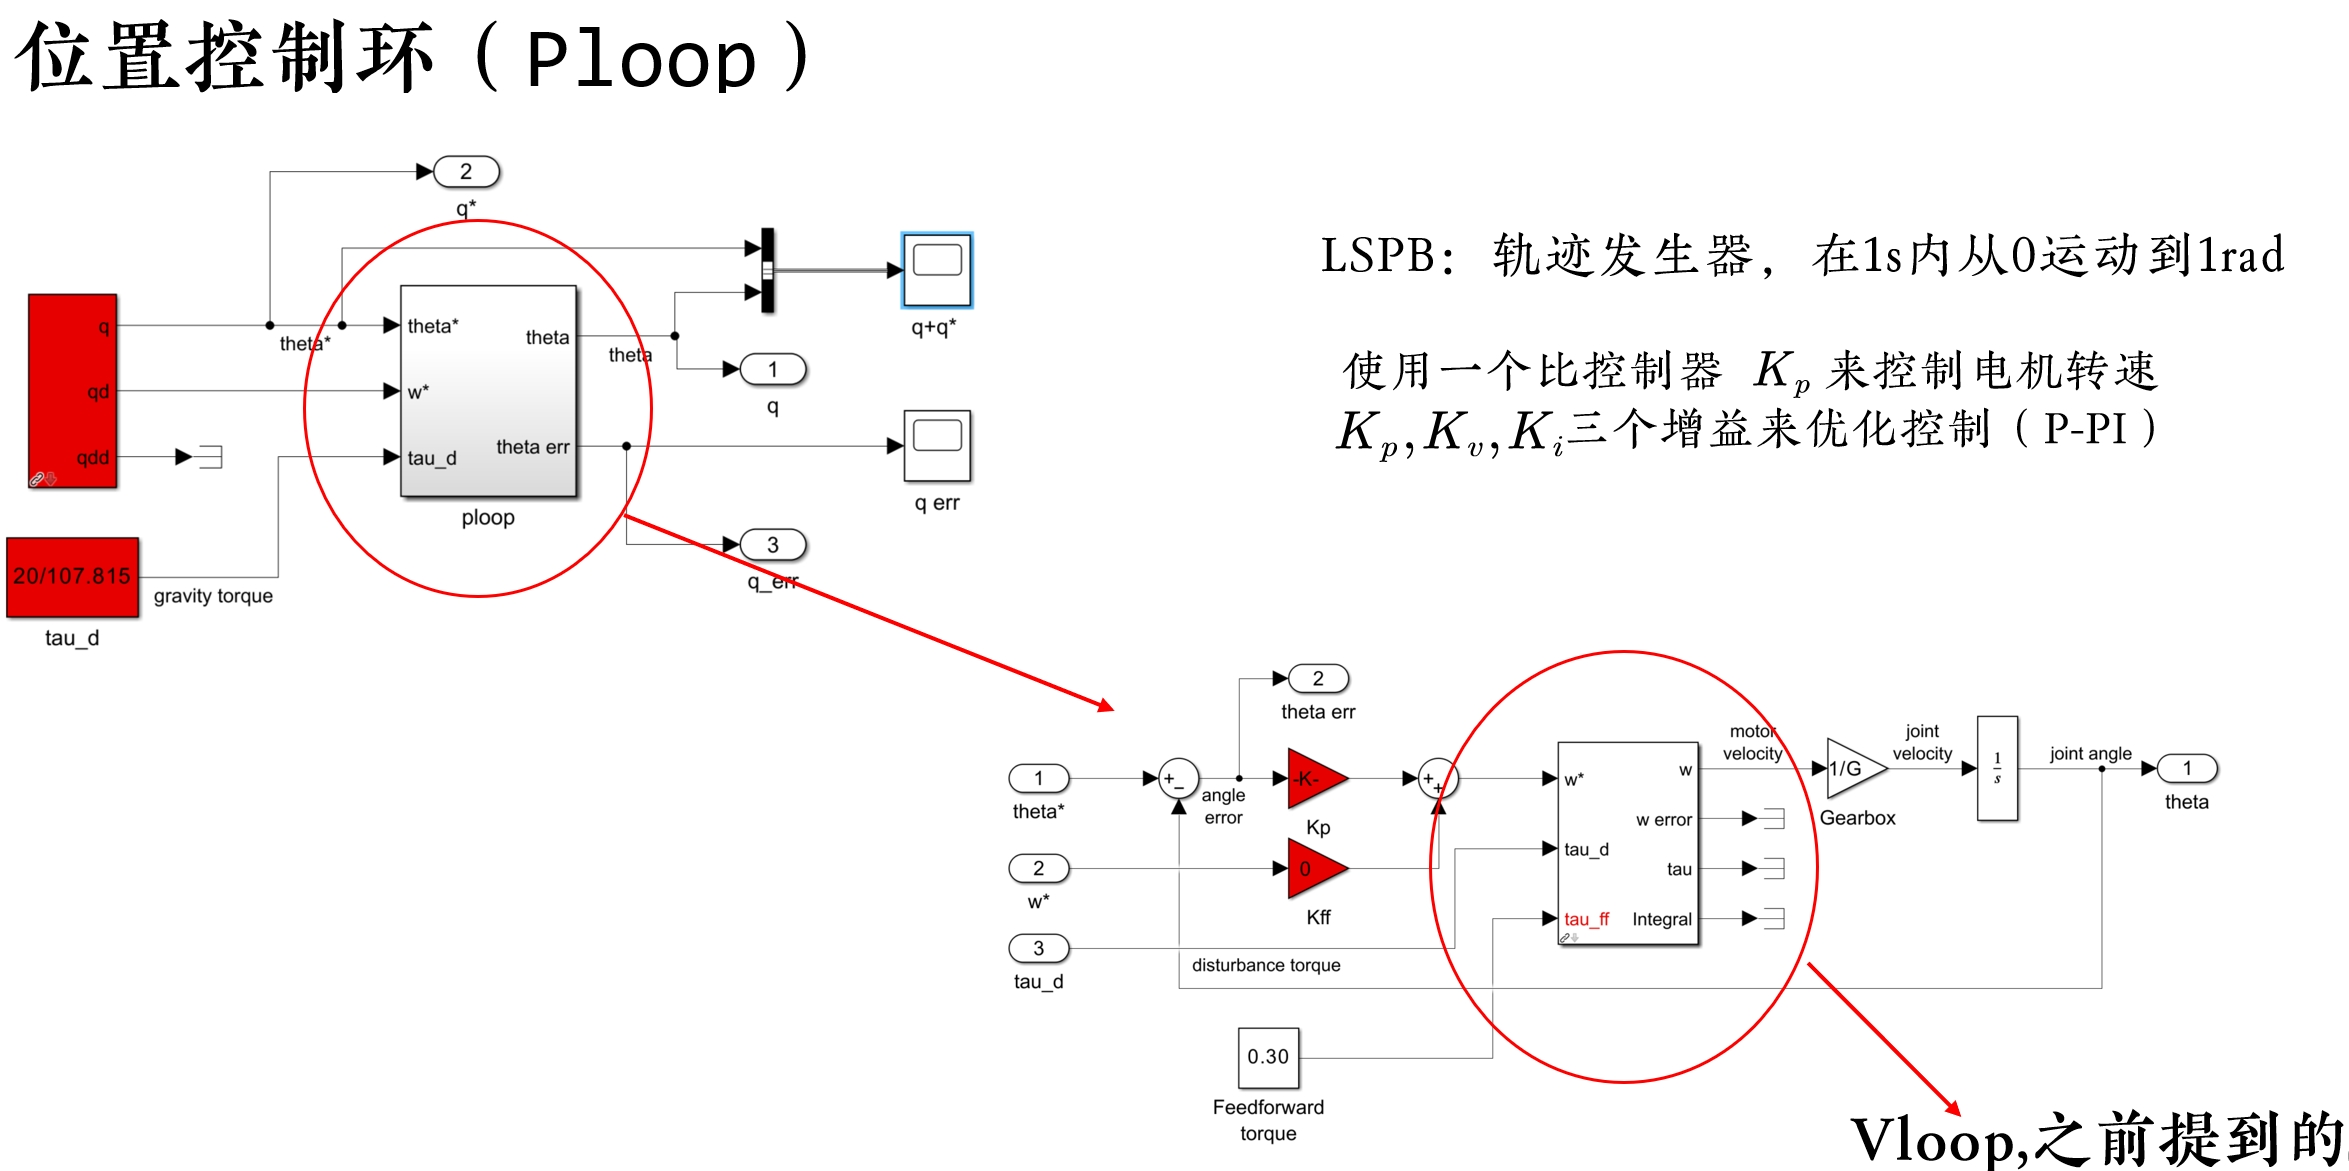
\includegraphics[width=\textwidth]{Image/ploop.png}
    \caption{总集成的位置-速度环控制系统}
    \label{fig:39}
\end{figure}

测试这个装置,如图\ref{fig:40}所示。左侧的图是只使用比例控制的情况,类似于速度环内的控制,我们添加一项期望速度的前馈,可以得到良好的跟踪效果。

\begin{figure}[htbp]
    \centering
    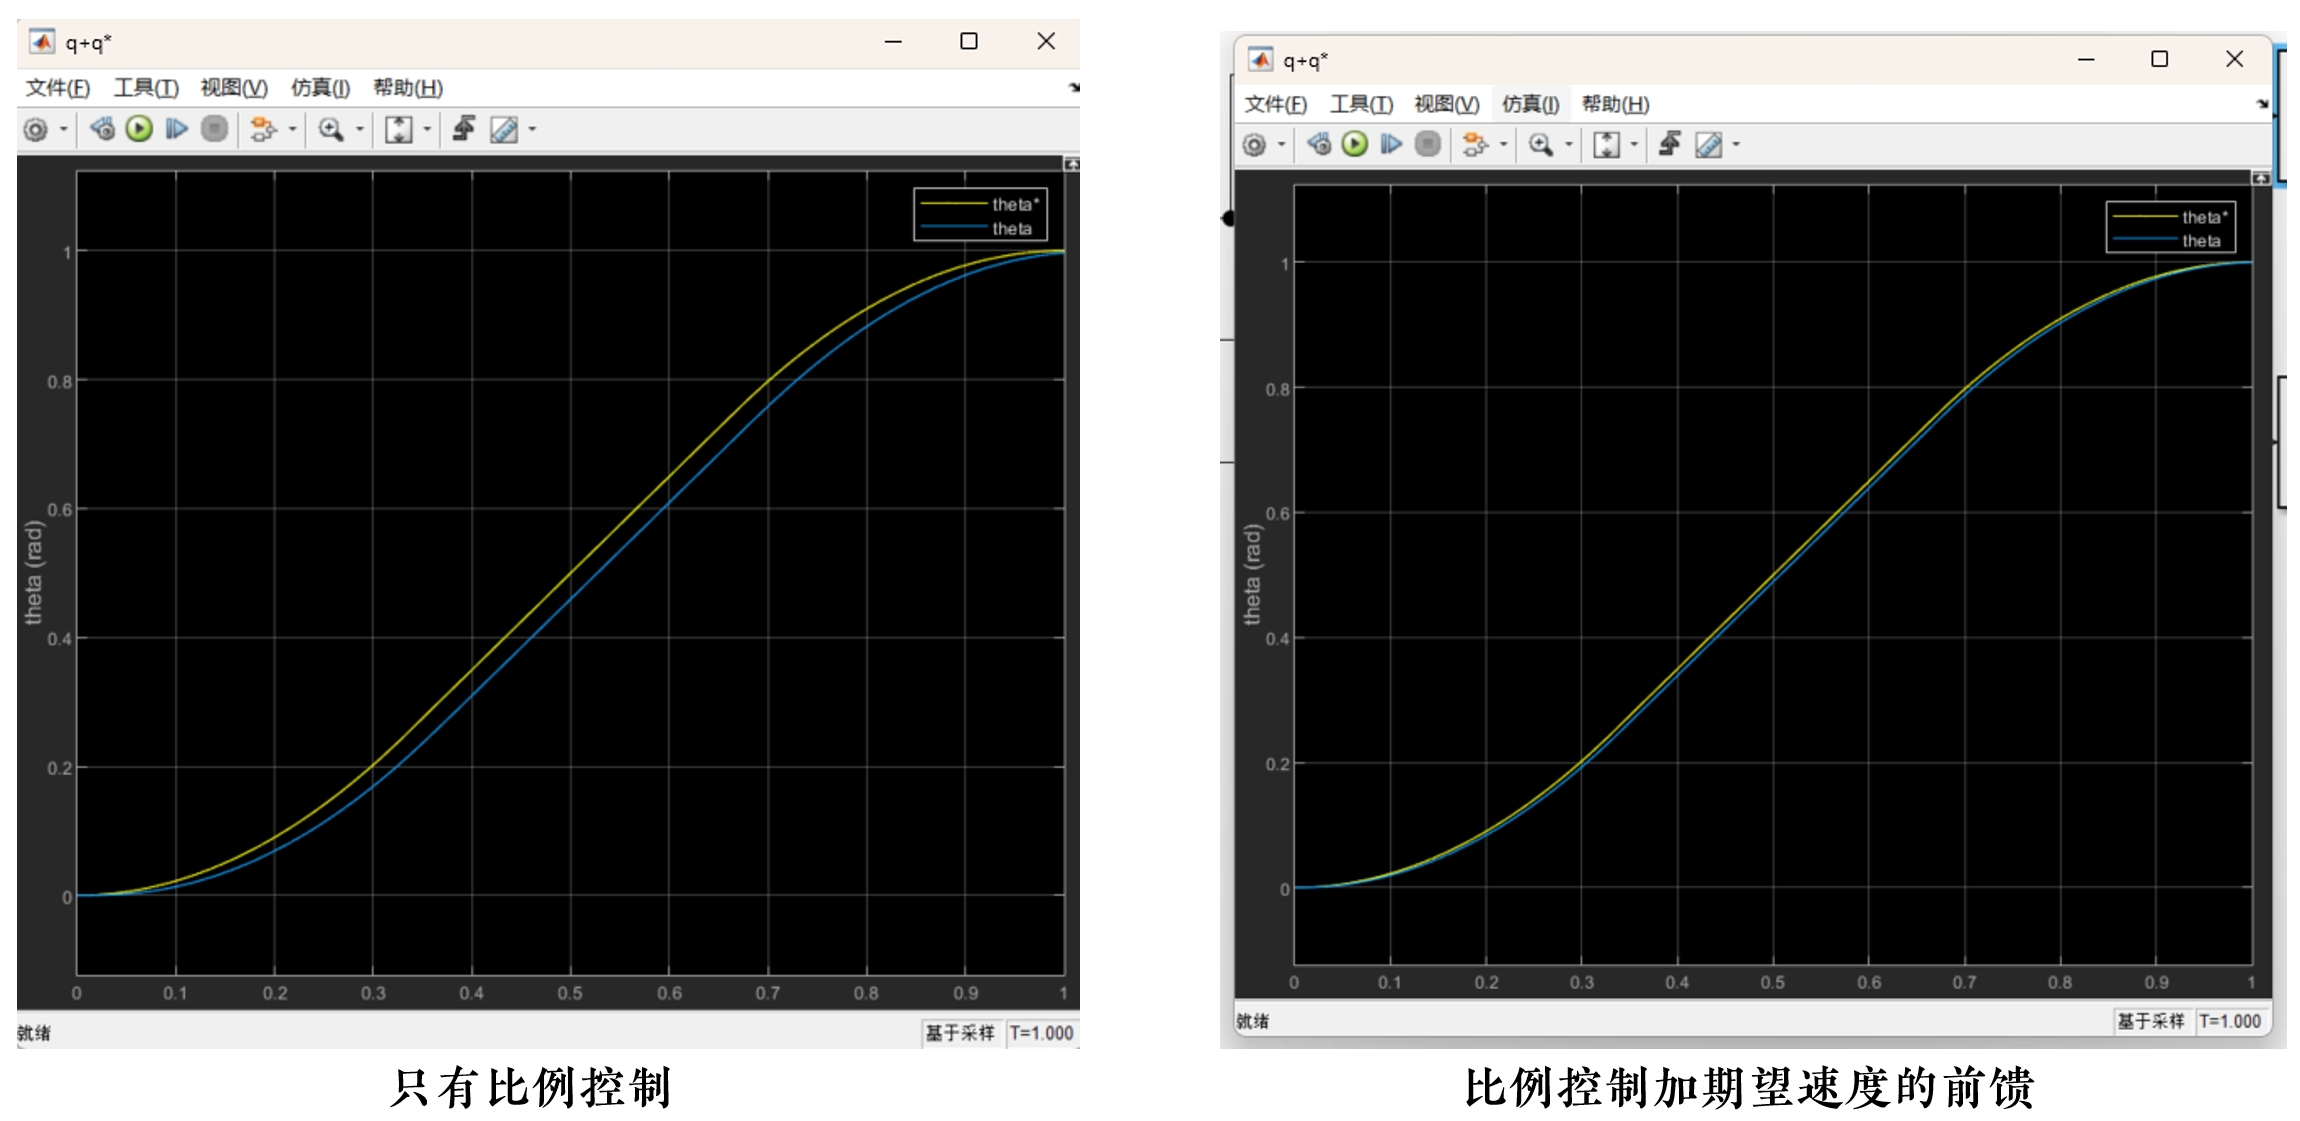
\includegraphics[width=\textwidth]{Image/fig43.png}
    \caption{位置环控制系统测试}
    \label{fig:40}
\end{figure}

至此,控制部分的工作我们组就做了这些。虽然有限的课程内容里我们对这个机器人的控制所学不多,但它属实是一门充满了挑战、充满了未知的任务。我想这些工作也是对我们所学的一个完美谢幕,愿这份热情在心中永不熄灭,生生不息。